\documentclass[12pt, a4paper]{article}
\usepackage{../notesheets}
%%%%%%%%%%%%%%%%%%%%%%%%%%%%%%%%%%%%%%%%%%%%%%%%%%
\author{Math 1220}
\title{Notesheet. Section 7.5: Surfaces of Revolution}
\date{}

\begin{document}
\maketitle
\nameline
%%%%%%%%%%%%%%%%%%%%%%%%%%%%%%%%%%%%%%%%%%%%%%%%%%
\begin{defi}
  A \de{solid of revolution} is \\
  
  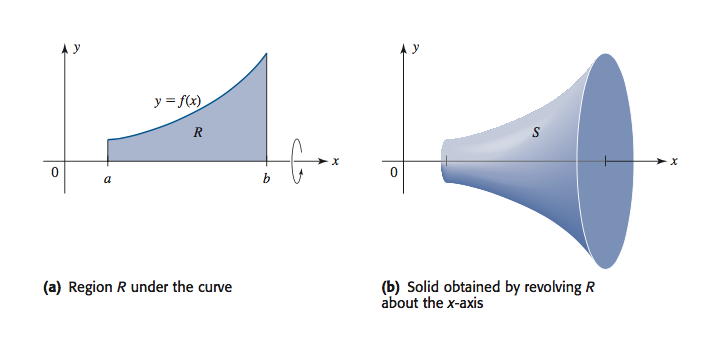
\includegraphics[scale=0.5]{images/surface-of-revolution}
\end{defi}
\begin{ex}
  We try to approximate the volume of a sphere by looking at the
  surface of revolution given by rotating the region under \(f(x) =
  \sqrt{r^2-x^2}\) (a semicircle) on \([-r,r]\).
  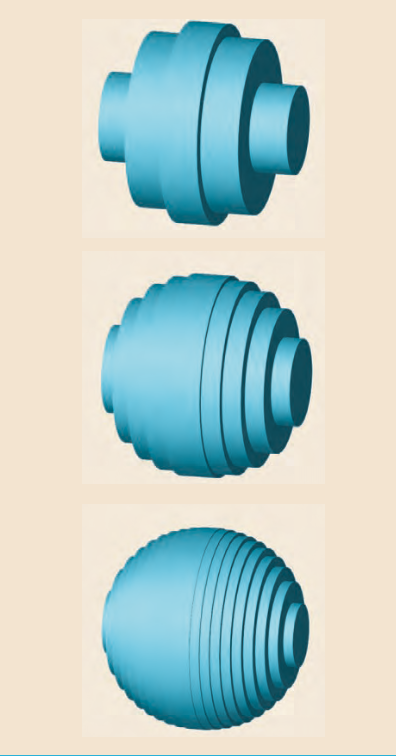
\includegraphics[scale=0.3]{images/approximating-volume-of-sphere}
\end{ex}
\begin{thrm}
  The volume \(V\) of the solid of revolution obtained by revolving
  the region below the graph of a nonnegative function \(y=f(x)\) from
  \(x=a\) to \(x=b\) about the \(x\)-axis is \[
    V = \hspace{1in}
  \]
\end{thrm}
\vspace{-0.5in}
\begin{ex}
  Compute the volume of the following solids of revolution.
  \begin{enumerate}
  \item Let \(f(x) = \frac{1}{3}x\) and rotate the area under the
    function from \([0,3]\) around the \(x\)-axis.
    \vspace{2in}
  \item Let \(f(x) = 4\) and rotate the area under the function from
    \([0,7]\) around the \(x\)-axis.
  \end{enumerate}
\end{ex}
\begin{thrm}
  Let \(R\) be a region bounded by the curves \(y=f(x)\) and
  \(y=g(x)\) from \(x=a\) to \(x=b\). Then, the volume \(V\) of the
  solid of revolution obtained by revolving \(R\) about the
  \(x\)-axis is give by \[
    V = \hspace{1in}
  \]
  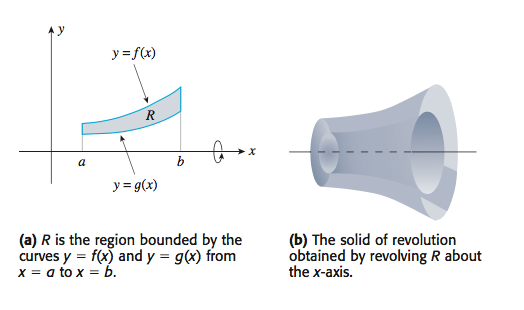
\includegraphics[scale=0.5]{images/surface-of-revolution2}
\end{thrm}
%%%%%%%%%%%%%%%%%%%%%%%%%%%%%%%%%%%%%%%%%%%%%%%%%% 
\end{document}
